% Created by tikzDevice version 0.12.3.1 on 2022-04-16 08:32:44
% !TEX encoding = UTF-8 Unicode
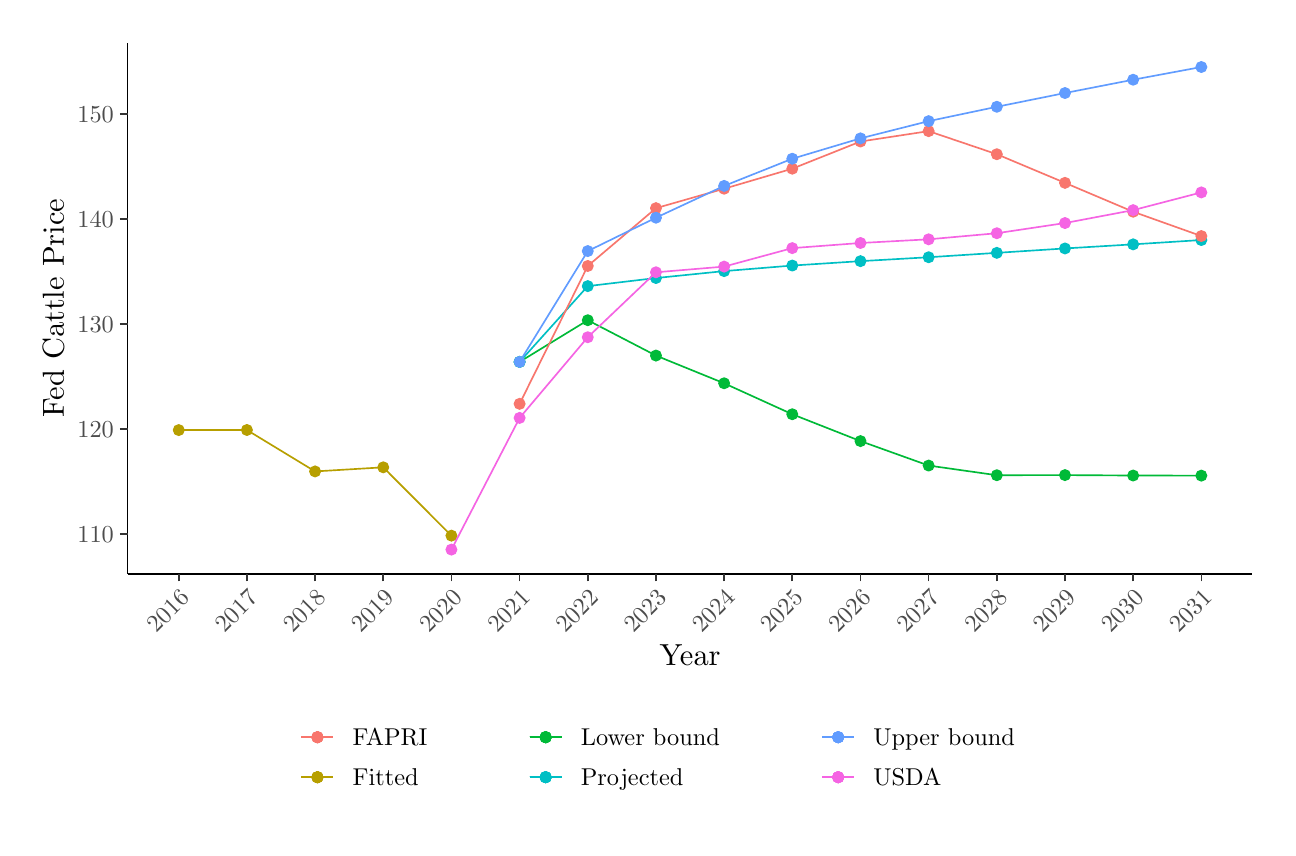
\begin{tikzpicture}[x=1pt,y=1pt]
\definecolor{fillColor}{RGB}{255,255,255}
\path[use as bounding box,fill=fillColor,fill opacity=0.00] (0,0) rectangle (448.07,289.08);
\begin{scope}
\path[clip] (  0.00,  0.00) rectangle (448.07,289.08);
\definecolor{drawColor}{RGB}{255,255,255}
\definecolor{fillColor}{RGB}{255,255,255}

\path[draw=drawColor,line width= 0.6pt,line join=round,line cap=round,fill=fillColor] (  0.00,  0.00) rectangle (448.07,289.08);
\end{scope}
\begin{scope}
\path[clip] ( 36.11, 91.76) rectangle (442.57,283.58);
\definecolor{fillColor}{RGB}{255,255,255}

\path[fill=fillColor] ( 36.11, 91.76) rectangle (442.57,283.58);
\definecolor{drawColor}{RGB}{183,159,0}

\path[draw=drawColor,line width= 0.6pt,line join=round] ( 54.59,143.67) --
	( 79.22,143.70) --
	(103.85,128.73) --
	(128.49,130.21) --
	(153.12,105.52);
\definecolor{fillColor}{RGB}{183,159,0}

\path[draw=drawColor,line width= 0.4pt,line join=round,line cap=round,fill=fillColor] ( 54.59,143.67) circle (  1.96);

\path[draw=drawColor,line width= 0.4pt,line join=round,line cap=round,fill=fillColor] ( 79.22,143.70) circle (  1.96);

\path[draw=drawColor,line width= 0.4pt,line join=round,line cap=round,fill=fillColor] (103.85,128.73) circle (  1.96);

\path[draw=drawColor,line width= 0.4pt,line join=round,line cap=round,fill=fillColor] (128.49,130.21) circle (  1.96);

\path[draw=drawColor,line width= 0.4pt,line join=round,line cap=round,fill=fillColor] (153.12,105.52) circle (  1.96);
\definecolor{drawColor}{RGB}{0,186,56}

\path[draw=drawColor,line width= 0.6pt,line join=round] (177.76,168.31) --
	(202.39,183.37) --
	(227.03,170.59) --
	(251.66,160.58) --
	(276.29,149.39) --
	(300.93,139.69) --
	(325.56,130.85) --
	(350.20,127.36) --
	(374.83,127.40) --
	(399.46,127.25) --
	(424.10,127.21);
\definecolor{fillColor}{RGB}{0,186,56}

\path[draw=drawColor,line width= 0.4pt,line join=round,line cap=round,fill=fillColor] (177.76,168.31) circle (  1.96);

\path[draw=drawColor,line width= 0.4pt,line join=round,line cap=round,fill=fillColor] (202.39,183.37) circle (  1.96);

\path[draw=drawColor,line width= 0.4pt,line join=round,line cap=round,fill=fillColor] (227.03,170.59) circle (  1.96);

\path[draw=drawColor,line width= 0.4pt,line join=round,line cap=round,fill=fillColor] (251.66,160.58) circle (  1.96);

\path[draw=drawColor,line width= 0.4pt,line join=round,line cap=round,fill=fillColor] (276.29,149.39) circle (  1.96);

\path[draw=drawColor,line width= 0.4pt,line join=round,line cap=round,fill=fillColor] (300.93,139.69) circle (  1.96);

\path[draw=drawColor,line width= 0.4pt,line join=round,line cap=round,fill=fillColor] (325.56,130.85) circle (  1.96);

\path[draw=drawColor,line width= 0.4pt,line join=round,line cap=round,fill=fillColor] (350.20,127.36) circle (  1.96);

\path[draw=drawColor,line width= 0.4pt,line join=round,line cap=round,fill=fillColor] (374.83,127.40) circle (  1.96);

\path[draw=drawColor,line width= 0.4pt,line join=round,line cap=round,fill=fillColor] (399.46,127.25) circle (  1.96);

\path[draw=drawColor,line width= 0.4pt,line join=round,line cap=round,fill=fillColor] (424.10,127.21) circle (  1.96);
\definecolor{drawColor}{RGB}{0,191,196}

\path[draw=drawColor,line width= 0.6pt,line join=round] (177.76,168.31) --
	(202.39,195.69) --
	(227.03,198.61) --
	(251.66,201.11) --
	(276.29,203.12) --
	(300.93,204.71) --
	(325.56,206.12) --
	(350.20,207.71) --
	(374.83,209.30) --
	(399.46,210.78) --
	(424.10,212.34);
\definecolor{fillColor}{RGB}{0,191,196}

\path[draw=drawColor,line width= 0.4pt,line join=round,line cap=round,fill=fillColor] (177.76,168.31) circle (  1.96);

\path[draw=drawColor,line width= 0.4pt,line join=round,line cap=round,fill=fillColor] (202.39,195.69) circle (  1.96);

\path[draw=drawColor,line width= 0.4pt,line join=round,line cap=round,fill=fillColor] (227.03,198.61) circle (  1.96);

\path[draw=drawColor,line width= 0.4pt,line join=round,line cap=round,fill=fillColor] (251.66,201.11) circle (  1.96);

\path[draw=drawColor,line width= 0.4pt,line join=round,line cap=round,fill=fillColor] (276.29,203.12) circle (  1.96);

\path[draw=drawColor,line width= 0.4pt,line join=round,line cap=round,fill=fillColor] (300.93,204.71) circle (  1.96);

\path[draw=drawColor,line width= 0.4pt,line join=round,line cap=round,fill=fillColor] (325.56,206.12) circle (  1.96);

\path[draw=drawColor,line width= 0.4pt,line join=round,line cap=round,fill=fillColor] (350.20,207.71) circle (  1.96);

\path[draw=drawColor,line width= 0.4pt,line join=round,line cap=round,fill=fillColor] (374.83,209.30) circle (  1.96);

\path[draw=drawColor,line width= 0.4pt,line join=round,line cap=round,fill=fillColor] (399.46,210.78) circle (  1.96);

\path[draw=drawColor,line width= 0.4pt,line join=round,line cap=round,fill=fillColor] (424.10,212.34) circle (  1.96);
\definecolor{drawColor}{RGB}{248,118,109}

\path[draw=drawColor,line width= 0.6pt,line join=round] (177.76,153.15) --
	(202.39,202.97) --
	(227.03,223.86) --
	(251.66,230.88) --
	(276.29,238.12) --
	(300.93,247.94) --
	(325.56,251.69) --
	(350.20,243.35) --
	(374.83,233.00) --
	(399.46,222.57) --
	(424.10,213.78);
\definecolor{fillColor}{RGB}{248,118,109}

\path[draw=drawColor,line width= 0.4pt,line join=round,line cap=round,fill=fillColor] (177.76,153.15) circle (  1.96);

\path[draw=drawColor,line width= 0.4pt,line join=round,line cap=round,fill=fillColor] (202.39,202.97) circle (  1.96);

\path[draw=drawColor,line width= 0.4pt,line join=round,line cap=round,fill=fillColor] (227.03,223.86) circle (  1.96);

\path[draw=drawColor,line width= 0.4pt,line join=round,line cap=round,fill=fillColor] (251.66,230.88) circle (  1.96);

\path[draw=drawColor,line width= 0.4pt,line join=round,line cap=round,fill=fillColor] (276.29,238.12) circle (  1.96);

\path[draw=drawColor,line width= 0.4pt,line join=round,line cap=round,fill=fillColor] (300.93,247.94) circle (  1.96);

\path[draw=drawColor,line width= 0.4pt,line join=round,line cap=round,fill=fillColor] (325.56,251.69) circle (  1.96);

\path[draw=drawColor,line width= 0.4pt,line join=round,line cap=round,fill=fillColor] (350.20,243.35) circle (  1.96);

\path[draw=drawColor,line width= 0.4pt,line join=round,line cap=round,fill=fillColor] (374.83,233.00) circle (  1.96);

\path[draw=drawColor,line width= 0.4pt,line join=round,line cap=round,fill=fillColor] (399.46,222.57) circle (  1.96);

\path[draw=drawColor,line width= 0.4pt,line join=round,line cap=round,fill=fillColor] (424.10,213.78) circle (  1.96);
\definecolor{drawColor}{RGB}{245,100,227}

\path[draw=drawColor,line width= 0.6pt,line join=round] (153.12,100.48) --
	(177.76,148.07) --
	(202.39,177.22) --
	(227.03,200.69) --
	(251.66,202.74) --
	(276.29,209.42) --
	(300.93,211.27) --
	(325.56,212.60) --
	(350.20,214.80) --
	(374.83,218.48) --
	(399.46,223.14) --
	(424.10,229.55);
\definecolor{fillColor}{RGB}{245,100,227}

\path[draw=drawColor,line width= 0.4pt,line join=round,line cap=round,fill=fillColor] (153.12,100.48) circle (  1.96);

\path[draw=drawColor,line width= 0.4pt,line join=round,line cap=round,fill=fillColor] (177.76,148.07) circle (  1.96);

\path[draw=drawColor,line width= 0.4pt,line join=round,line cap=round,fill=fillColor] (202.39,177.22) circle (  1.96);

\path[draw=drawColor,line width= 0.4pt,line join=round,line cap=round,fill=fillColor] (227.03,200.69) circle (  1.96);

\path[draw=drawColor,line width= 0.4pt,line join=round,line cap=round,fill=fillColor] (251.66,202.74) circle (  1.96);

\path[draw=drawColor,line width= 0.4pt,line join=round,line cap=round,fill=fillColor] (276.29,209.42) circle (  1.96);

\path[draw=drawColor,line width= 0.4pt,line join=round,line cap=round,fill=fillColor] (300.93,211.27) circle (  1.96);

\path[draw=drawColor,line width= 0.4pt,line join=round,line cap=round,fill=fillColor] (325.56,212.60) circle (  1.96);

\path[draw=drawColor,line width= 0.4pt,line join=round,line cap=round,fill=fillColor] (350.20,214.80) circle (  1.96);

\path[draw=drawColor,line width= 0.4pt,line join=round,line cap=round,fill=fillColor] (374.83,218.48) circle (  1.96);

\path[draw=drawColor,line width= 0.4pt,line join=round,line cap=round,fill=fillColor] (399.46,223.14) circle (  1.96);

\path[draw=drawColor,line width= 0.4pt,line join=round,line cap=round,fill=fillColor] (424.10,229.55) circle (  1.96);
\definecolor{drawColor}{RGB}{97,156,255}

\path[draw=drawColor,line width= 0.6pt,line join=round] (177.76,168.31) --
	(202.39,208.35) --
	(227.03,220.41) --
	(251.66,231.90) --
	(276.29,241.72) --
	(300.93,249.08) --
	(325.56,255.30) --
	(350.20,260.49) --
	(374.83,265.46) --
	(399.46,270.27) --
	(424.10,274.86);
\definecolor{fillColor}{RGB}{97,156,255}

\path[draw=drawColor,line width= 0.4pt,line join=round,line cap=round,fill=fillColor] (177.76,168.31) circle (  1.96);

\path[draw=drawColor,line width= 0.4pt,line join=round,line cap=round,fill=fillColor] (202.39,208.35) circle (  1.96);

\path[draw=drawColor,line width= 0.4pt,line join=round,line cap=round,fill=fillColor] (227.03,220.41) circle (  1.96);

\path[draw=drawColor,line width= 0.4pt,line join=round,line cap=round,fill=fillColor] (251.66,231.90) circle (  1.96);

\path[draw=drawColor,line width= 0.4pt,line join=round,line cap=round,fill=fillColor] (276.29,241.72) circle (  1.96);

\path[draw=drawColor,line width= 0.4pt,line join=round,line cap=round,fill=fillColor] (300.93,249.08) circle (  1.96);

\path[draw=drawColor,line width= 0.4pt,line join=round,line cap=round,fill=fillColor] (325.56,255.30) circle (  1.96);

\path[draw=drawColor,line width= 0.4pt,line join=round,line cap=round,fill=fillColor] (350.20,260.49) circle (  1.96);

\path[draw=drawColor,line width= 0.4pt,line join=round,line cap=round,fill=fillColor] (374.83,265.46) circle (  1.96);

\path[draw=drawColor,line width= 0.4pt,line join=round,line cap=round,fill=fillColor] (399.46,270.27) circle (  1.96);

\path[draw=drawColor,line width= 0.4pt,line join=round,line cap=round,fill=fillColor] (424.10,274.86) circle (  1.96);
\end{scope}
\begin{scope}
\path[clip] (  0.00,  0.00) rectangle (448.07,289.08);
\definecolor{drawColor}{RGB}{0,0,0}

\path[draw=drawColor,line width= 0.6pt,line join=round] ( 36.11, 91.76) --
	( 36.11,283.58);
\end{scope}
\begin{scope}
\path[clip] (  0.00,  0.00) rectangle (448.07,289.08);
\definecolor{drawColor}{gray}{0.30}

\node[text=drawColor,anchor=base east,inner sep=0pt, outer sep=0pt, scale=  0.88] at ( 31.16,103.10) {110};

\node[text=drawColor,anchor=base east,inner sep=0pt, outer sep=0pt, scale=  0.88] at ( 31.16,141.02) {120};

\node[text=drawColor,anchor=base east,inner sep=0pt, outer sep=0pt, scale=  0.88] at ( 31.16,178.93) {130};

\node[text=drawColor,anchor=base east,inner sep=0pt, outer sep=0pt, scale=  0.88] at ( 31.16,216.85) {140};

\node[text=drawColor,anchor=base east,inner sep=0pt, outer sep=0pt, scale=  0.88] at ( 31.16,254.77) {150};
\end{scope}
\begin{scope}
\path[clip] (  0.00,  0.00) rectangle (448.07,289.08);
\definecolor{drawColor}{gray}{0.20}

\path[draw=drawColor,line width= 0.6pt,line join=round] ( 33.36,106.13) --
	( 36.11,106.13);

\path[draw=drawColor,line width= 0.6pt,line join=round] ( 33.36,144.05) --
	( 36.11,144.05);

\path[draw=drawColor,line width= 0.6pt,line join=round] ( 33.36,181.96) --
	( 36.11,181.96);

\path[draw=drawColor,line width= 0.6pt,line join=round] ( 33.36,219.88) --
	( 36.11,219.88);

\path[draw=drawColor,line width= 0.6pt,line join=round] ( 33.36,257.80) --
	( 36.11,257.80);
\end{scope}
\begin{scope}
\path[clip] (  0.00,  0.00) rectangle (448.07,289.08);
\definecolor{drawColor}{RGB}{0,0,0}

\path[draw=drawColor,line width= 0.6pt,line join=round] ( 36.11, 91.76) --
	(442.57, 91.76);
\end{scope}
\begin{scope}
\path[clip] (  0.00,  0.00) rectangle (448.07,289.08);
\definecolor{drawColor}{gray}{0.20}

\path[draw=drawColor,line width= 0.6pt,line join=round] ( 54.59, 89.01) --
	( 54.59, 91.76);

\path[draw=drawColor,line width= 0.6pt,line join=round] ( 79.22, 89.01) --
	( 79.22, 91.76);

\path[draw=drawColor,line width= 0.6pt,line join=round] (103.85, 89.01) --
	(103.85, 91.76);

\path[draw=drawColor,line width= 0.6pt,line join=round] (128.49, 89.01) --
	(128.49, 91.76);

\path[draw=drawColor,line width= 0.6pt,line join=round] (153.12, 89.01) --
	(153.12, 91.76);

\path[draw=drawColor,line width= 0.6pt,line join=round] (177.76, 89.01) --
	(177.76, 91.76);

\path[draw=drawColor,line width= 0.6pt,line join=round] (202.39, 89.01) --
	(202.39, 91.76);

\path[draw=drawColor,line width= 0.6pt,line join=round] (227.03, 89.01) --
	(227.03, 91.76);

\path[draw=drawColor,line width= 0.6pt,line join=round] (251.66, 89.01) --
	(251.66, 91.76);

\path[draw=drawColor,line width= 0.6pt,line join=round] (276.29, 89.01) --
	(276.29, 91.76);

\path[draw=drawColor,line width= 0.6pt,line join=round] (300.93, 89.01) --
	(300.93, 91.76);

\path[draw=drawColor,line width= 0.6pt,line join=round] (325.56, 89.01) --
	(325.56, 91.76);

\path[draw=drawColor,line width= 0.6pt,line join=round] (350.20, 89.01) --
	(350.20, 91.76);

\path[draw=drawColor,line width= 0.6pt,line join=round] (374.83, 89.01) --
	(374.83, 91.76);

\path[draw=drawColor,line width= 0.6pt,line join=round] (399.46, 89.01) --
	(399.46, 91.76);

\path[draw=drawColor,line width= 0.6pt,line join=round] (424.10, 89.01) --
	(424.10, 91.76);
\end{scope}
\begin{scope}
\path[clip] (  0.00,  0.00) rectangle (448.07,289.08);
\definecolor{drawColor}{gray}{0.30}

\node[text=drawColor,rotate= 45.00,anchor=base east,inner sep=0pt, outer sep=0pt, scale=  0.88] at ( 58.87, 82.52) {2016};

\node[text=drawColor,rotate= 45.00,anchor=base east,inner sep=0pt, outer sep=0pt, scale=  0.88] at ( 83.51, 82.52) {2017};

\node[text=drawColor,rotate= 45.00,anchor=base east,inner sep=0pt, outer sep=0pt, scale=  0.88] at (108.14, 82.52) {2018};

\node[text=drawColor,rotate= 45.00,anchor=base east,inner sep=0pt, outer sep=0pt, scale=  0.88] at (132.77, 82.52) {2019};

\node[text=drawColor,rotate= 45.00,anchor=base east,inner sep=0pt, outer sep=0pt, scale=  0.88] at (157.41, 82.52) {2020};

\node[text=drawColor,rotate= 45.00,anchor=base east,inner sep=0pt, outer sep=0pt, scale=  0.88] at (182.04, 82.52) {2021};

\node[text=drawColor,rotate= 45.00,anchor=base east,inner sep=0pt, outer sep=0pt, scale=  0.88] at (206.68, 82.52) {2022};

\node[text=drawColor,rotate= 45.00,anchor=base east,inner sep=0pt, outer sep=0pt, scale=  0.88] at (231.31, 82.52) {2023};

\node[text=drawColor,rotate= 45.00,anchor=base east,inner sep=0pt, outer sep=0pt, scale=  0.88] at (255.95, 82.52) {2024};

\node[text=drawColor,rotate= 45.00,anchor=base east,inner sep=0pt, outer sep=0pt, scale=  0.88] at (280.58, 82.52) {2025};

\node[text=drawColor,rotate= 45.00,anchor=base east,inner sep=0pt, outer sep=0pt, scale=  0.88] at (305.21, 82.52) {2026};

\node[text=drawColor,rotate= 45.00,anchor=base east,inner sep=0pt, outer sep=0pt, scale=  0.88] at (329.85, 82.52) {2027};

\node[text=drawColor,rotate= 45.00,anchor=base east,inner sep=0pt, outer sep=0pt, scale=  0.88] at (354.48, 82.52) {2028};

\node[text=drawColor,rotate= 45.00,anchor=base east,inner sep=0pt, outer sep=0pt, scale=  0.88] at (379.12, 82.52) {2029};

\node[text=drawColor,rotate= 45.00,anchor=base east,inner sep=0pt, outer sep=0pt, scale=  0.88] at (403.75, 82.52) {2030};

\node[text=drawColor,rotate= 45.00,anchor=base east,inner sep=0pt, outer sep=0pt, scale=  0.88] at (428.38, 82.52) {2031};
\end{scope}
\begin{scope}
\path[clip] (  0.00,  0.00) rectangle (448.07,289.08);
\definecolor{drawColor}{RGB}{0,0,0}

\node[text=drawColor,anchor=base,inner sep=0pt, outer sep=0pt, scale=  1.10] at (239.34, 58.55) {Year};
\end{scope}
\begin{scope}
\path[clip] (  0.00,  0.00) rectangle (448.07,289.08);
\definecolor{drawColor}{RGB}{0,0,0}

\node[text=drawColor,rotate= 90.00,anchor=base,inner sep=0pt, outer sep=0pt, scale=  1.10] at ( 13.08,187.67) {Fed Cattle Price};
\end{scope}
\begin{scope}
\path[clip] (  0.00,  0.00) rectangle (448.07,289.08);
\definecolor{fillColor}{RGB}{255,255,255}

\path[fill=fillColor] ( 86.49,  5.50) rectangle (392.20, 45.41);
\end{scope}
\begin{scope}
\path[clip] (  0.00,  0.00) rectangle (448.07,289.08);
\definecolor{drawColor}{RGB}{248,118,109}

\path[draw=drawColor,line width= 0.6pt,line join=round] ( 98.93, 32.68) -- (110.49, 32.68);
\end{scope}
\begin{scope}
\path[clip] (  0.00,  0.00) rectangle (448.07,289.08);
\definecolor{drawColor}{RGB}{248,118,109}
\definecolor{fillColor}{RGB}{248,118,109}

\path[draw=drawColor,line width= 0.4pt,line join=round,line cap=round,fill=fillColor] (104.71, 32.68) circle (  1.96);
\end{scope}
\begin{scope}
\path[clip] (  0.00,  0.00) rectangle (448.07,289.08);
\definecolor{drawColor}{RGB}{248,118,109}

\path[draw=drawColor,line width= 0.6pt,line join=round] ( 98.93, 32.68) -- (110.49, 32.68);
\end{scope}
\begin{scope}
\path[clip] (  0.00,  0.00) rectangle (448.07,289.08);
\definecolor{drawColor}{RGB}{248,118,109}
\definecolor{fillColor}{RGB}{248,118,109}

\path[draw=drawColor,line width= 0.4pt,line join=round,line cap=round,fill=fillColor] (104.71, 32.68) circle (  1.96);
\end{scope}
\begin{scope}
\path[clip] (  0.00,  0.00) rectangle (448.07,289.08);
\definecolor{drawColor}{RGB}{248,118,109}

\path[draw=drawColor,line width= 0.6pt,line join=round] ( 98.93, 32.68) -- (110.49, 32.68);
\end{scope}
\begin{scope}
\path[clip] (  0.00,  0.00) rectangle (448.07,289.08);
\definecolor{drawColor}{RGB}{248,118,109}
\definecolor{fillColor}{RGB}{248,118,109}

\path[draw=drawColor,line width= 0.4pt,line join=round,line cap=round,fill=fillColor] (104.71, 32.68) circle (  1.96);
\end{scope}
\begin{scope}
\path[clip] (  0.00,  0.00) rectangle (448.07,289.08);
\definecolor{drawColor}{RGB}{248,118,109}

\path[draw=drawColor,line width= 0.6pt,line join=round] ( 98.93, 32.68) -- (110.49, 32.68);
\end{scope}
\begin{scope}
\path[clip] (  0.00,  0.00) rectangle (448.07,289.08);
\definecolor{drawColor}{RGB}{248,118,109}
\definecolor{fillColor}{RGB}{248,118,109}

\path[draw=drawColor,line width= 0.4pt,line join=round,line cap=round,fill=fillColor] (104.71, 32.68) circle (  1.96);
\end{scope}
\begin{scope}
\path[clip] (  0.00,  0.00) rectangle (448.07,289.08);
\definecolor{drawColor}{RGB}{248,118,109}

\path[draw=drawColor,line width= 0.6pt,line join=round] ( 98.93, 32.68) -- (110.49, 32.68);
\end{scope}
\begin{scope}
\path[clip] (  0.00,  0.00) rectangle (448.07,289.08);
\definecolor{drawColor}{RGB}{248,118,109}
\definecolor{fillColor}{RGB}{248,118,109}

\path[draw=drawColor,line width= 0.4pt,line join=round,line cap=round,fill=fillColor] (104.71, 32.68) circle (  1.96);
\end{scope}
\begin{scope}
\path[clip] (  0.00,  0.00) rectangle (448.07,289.08);
\definecolor{drawColor}{RGB}{248,118,109}

\path[draw=drawColor,line width= 0.6pt,line join=round] ( 98.93, 32.68) -- (110.49, 32.68);
\end{scope}
\begin{scope}
\path[clip] (  0.00,  0.00) rectangle (448.07,289.08);
\definecolor{drawColor}{RGB}{248,118,109}
\definecolor{fillColor}{RGB}{248,118,109}

\path[draw=drawColor,line width= 0.4pt,line join=round,line cap=round,fill=fillColor] (104.71, 32.68) circle (  1.96);
\end{scope}
\begin{scope}
\path[clip] (  0.00,  0.00) rectangle (448.07,289.08);
\definecolor{drawColor}{RGB}{183,159,0}

\path[draw=drawColor,line width= 0.6pt,line join=round] ( 98.93, 18.23) -- (110.49, 18.23);
\end{scope}
\begin{scope}
\path[clip] (  0.00,  0.00) rectangle (448.07,289.08);
\definecolor{drawColor}{RGB}{183,159,0}
\definecolor{fillColor}{RGB}{183,159,0}

\path[draw=drawColor,line width= 0.4pt,line join=round,line cap=round,fill=fillColor] (104.71, 18.23) circle (  1.96);
\end{scope}
\begin{scope}
\path[clip] (  0.00,  0.00) rectangle (448.07,289.08);
\definecolor{drawColor}{RGB}{183,159,0}

\path[draw=drawColor,line width= 0.6pt,line join=round] ( 98.93, 18.23) -- (110.49, 18.23);
\end{scope}
\begin{scope}
\path[clip] (  0.00,  0.00) rectangle (448.07,289.08);
\definecolor{drawColor}{RGB}{183,159,0}
\definecolor{fillColor}{RGB}{183,159,0}

\path[draw=drawColor,line width= 0.4pt,line join=round,line cap=round,fill=fillColor] (104.71, 18.23) circle (  1.96);
\end{scope}
\begin{scope}
\path[clip] (  0.00,  0.00) rectangle (448.07,289.08);
\definecolor{drawColor}{RGB}{183,159,0}

\path[draw=drawColor,line width= 0.6pt,line join=round] ( 98.93, 18.23) -- (110.49, 18.23);
\end{scope}
\begin{scope}
\path[clip] (  0.00,  0.00) rectangle (448.07,289.08);
\definecolor{drawColor}{RGB}{183,159,0}
\definecolor{fillColor}{RGB}{183,159,0}

\path[draw=drawColor,line width= 0.4pt,line join=round,line cap=round,fill=fillColor] (104.71, 18.23) circle (  1.96);
\end{scope}
\begin{scope}
\path[clip] (  0.00,  0.00) rectangle (448.07,289.08);
\definecolor{drawColor}{RGB}{183,159,0}

\path[draw=drawColor,line width= 0.6pt,line join=round] ( 98.93, 18.23) -- (110.49, 18.23);
\end{scope}
\begin{scope}
\path[clip] (  0.00,  0.00) rectangle (448.07,289.08);
\definecolor{drawColor}{RGB}{183,159,0}
\definecolor{fillColor}{RGB}{183,159,0}

\path[draw=drawColor,line width= 0.4pt,line join=round,line cap=round,fill=fillColor] (104.71, 18.23) circle (  1.96);
\end{scope}
\begin{scope}
\path[clip] (  0.00,  0.00) rectangle (448.07,289.08);
\definecolor{drawColor}{RGB}{183,159,0}

\path[draw=drawColor,line width= 0.6pt,line join=round] ( 98.93, 18.23) -- (110.49, 18.23);
\end{scope}
\begin{scope}
\path[clip] (  0.00,  0.00) rectangle (448.07,289.08);
\definecolor{drawColor}{RGB}{183,159,0}
\definecolor{fillColor}{RGB}{183,159,0}

\path[draw=drawColor,line width= 0.4pt,line join=round,line cap=round,fill=fillColor] (104.71, 18.23) circle (  1.96);
\end{scope}
\begin{scope}
\path[clip] (  0.00,  0.00) rectangle (448.07,289.08);
\definecolor{drawColor}{RGB}{183,159,0}

\path[draw=drawColor,line width= 0.6pt,line join=round] ( 98.93, 18.23) -- (110.49, 18.23);
\end{scope}
\begin{scope}
\path[clip] (  0.00,  0.00) rectangle (448.07,289.08);
\definecolor{drawColor}{RGB}{183,159,0}
\definecolor{fillColor}{RGB}{183,159,0}

\path[draw=drawColor,line width= 0.4pt,line join=round,line cap=round,fill=fillColor] (104.71, 18.23) circle (  1.96);
\end{scope}
\begin{scope}
\path[clip] (  0.00,  0.00) rectangle (448.07,289.08);
\definecolor{drawColor}{RGB}{0,186,56}

\path[draw=drawColor,line width= 0.6pt,line join=round] (181.39, 32.68) -- (192.95, 32.68);
\end{scope}
\begin{scope}
\path[clip] (  0.00,  0.00) rectangle (448.07,289.08);
\definecolor{drawColor}{RGB}{0,186,56}
\definecolor{fillColor}{RGB}{0,186,56}

\path[draw=drawColor,line width= 0.4pt,line join=round,line cap=round,fill=fillColor] (187.17, 32.68) circle (  1.96);
\end{scope}
\begin{scope}
\path[clip] (  0.00,  0.00) rectangle (448.07,289.08);
\definecolor{drawColor}{RGB}{0,186,56}

\path[draw=drawColor,line width= 0.6pt,line join=round] (181.39, 32.68) -- (192.95, 32.68);
\end{scope}
\begin{scope}
\path[clip] (  0.00,  0.00) rectangle (448.07,289.08);
\definecolor{drawColor}{RGB}{0,186,56}
\definecolor{fillColor}{RGB}{0,186,56}

\path[draw=drawColor,line width= 0.4pt,line join=round,line cap=round,fill=fillColor] (187.17, 32.68) circle (  1.96);
\end{scope}
\begin{scope}
\path[clip] (  0.00,  0.00) rectangle (448.07,289.08);
\definecolor{drawColor}{RGB}{0,186,56}

\path[draw=drawColor,line width= 0.6pt,line join=round] (181.39, 32.68) -- (192.95, 32.68);
\end{scope}
\begin{scope}
\path[clip] (  0.00,  0.00) rectangle (448.07,289.08);
\definecolor{drawColor}{RGB}{0,186,56}
\definecolor{fillColor}{RGB}{0,186,56}

\path[draw=drawColor,line width= 0.4pt,line join=round,line cap=round,fill=fillColor] (187.17, 32.68) circle (  1.96);
\end{scope}
\begin{scope}
\path[clip] (  0.00,  0.00) rectangle (448.07,289.08);
\definecolor{drawColor}{RGB}{0,186,56}

\path[draw=drawColor,line width= 0.6pt,line join=round] (181.39, 32.68) -- (192.95, 32.68);
\end{scope}
\begin{scope}
\path[clip] (  0.00,  0.00) rectangle (448.07,289.08);
\definecolor{drawColor}{RGB}{0,186,56}
\definecolor{fillColor}{RGB}{0,186,56}

\path[draw=drawColor,line width= 0.4pt,line join=round,line cap=round,fill=fillColor] (187.17, 32.68) circle (  1.96);
\end{scope}
\begin{scope}
\path[clip] (  0.00,  0.00) rectangle (448.07,289.08);
\definecolor{drawColor}{RGB}{0,186,56}

\path[draw=drawColor,line width= 0.6pt,line join=round] (181.39, 32.68) -- (192.95, 32.68);
\end{scope}
\begin{scope}
\path[clip] (  0.00,  0.00) rectangle (448.07,289.08);
\definecolor{drawColor}{RGB}{0,186,56}
\definecolor{fillColor}{RGB}{0,186,56}

\path[draw=drawColor,line width= 0.4pt,line join=round,line cap=round,fill=fillColor] (187.17, 32.68) circle (  1.96);
\end{scope}
\begin{scope}
\path[clip] (  0.00,  0.00) rectangle (448.07,289.08);
\definecolor{drawColor}{RGB}{0,186,56}

\path[draw=drawColor,line width= 0.6pt,line join=round] (181.39, 32.68) -- (192.95, 32.68);
\end{scope}
\begin{scope}
\path[clip] (  0.00,  0.00) rectangle (448.07,289.08);
\definecolor{drawColor}{RGB}{0,186,56}
\definecolor{fillColor}{RGB}{0,186,56}

\path[draw=drawColor,line width= 0.4pt,line join=round,line cap=round,fill=fillColor] (187.17, 32.68) circle (  1.96);
\end{scope}
\begin{scope}
\path[clip] (  0.00,  0.00) rectangle (448.07,289.08);
\definecolor{drawColor}{RGB}{0,191,196}

\path[draw=drawColor,line width= 0.6pt,line join=round] (181.39, 18.23) -- (192.95, 18.23);
\end{scope}
\begin{scope}
\path[clip] (  0.00,  0.00) rectangle (448.07,289.08);
\definecolor{drawColor}{RGB}{0,191,196}
\definecolor{fillColor}{RGB}{0,191,196}

\path[draw=drawColor,line width= 0.4pt,line join=round,line cap=round,fill=fillColor] (187.17, 18.23) circle (  1.96);
\end{scope}
\begin{scope}
\path[clip] (  0.00,  0.00) rectangle (448.07,289.08);
\definecolor{drawColor}{RGB}{0,191,196}

\path[draw=drawColor,line width= 0.6pt,line join=round] (181.39, 18.23) -- (192.95, 18.23);
\end{scope}
\begin{scope}
\path[clip] (  0.00,  0.00) rectangle (448.07,289.08);
\definecolor{drawColor}{RGB}{0,191,196}
\definecolor{fillColor}{RGB}{0,191,196}

\path[draw=drawColor,line width= 0.4pt,line join=round,line cap=round,fill=fillColor] (187.17, 18.23) circle (  1.96);
\end{scope}
\begin{scope}
\path[clip] (  0.00,  0.00) rectangle (448.07,289.08);
\definecolor{drawColor}{RGB}{0,191,196}

\path[draw=drawColor,line width= 0.6pt,line join=round] (181.39, 18.23) -- (192.95, 18.23);
\end{scope}
\begin{scope}
\path[clip] (  0.00,  0.00) rectangle (448.07,289.08);
\definecolor{drawColor}{RGB}{0,191,196}
\definecolor{fillColor}{RGB}{0,191,196}

\path[draw=drawColor,line width= 0.4pt,line join=round,line cap=round,fill=fillColor] (187.17, 18.23) circle (  1.96);
\end{scope}
\begin{scope}
\path[clip] (  0.00,  0.00) rectangle (448.07,289.08);
\definecolor{drawColor}{RGB}{0,191,196}

\path[draw=drawColor,line width= 0.6pt,line join=round] (181.39, 18.23) -- (192.95, 18.23);
\end{scope}
\begin{scope}
\path[clip] (  0.00,  0.00) rectangle (448.07,289.08);
\definecolor{drawColor}{RGB}{0,191,196}
\definecolor{fillColor}{RGB}{0,191,196}

\path[draw=drawColor,line width= 0.4pt,line join=round,line cap=round,fill=fillColor] (187.17, 18.23) circle (  1.96);
\end{scope}
\begin{scope}
\path[clip] (  0.00,  0.00) rectangle (448.07,289.08);
\definecolor{drawColor}{RGB}{0,191,196}

\path[draw=drawColor,line width= 0.6pt,line join=round] (181.39, 18.23) -- (192.95, 18.23);
\end{scope}
\begin{scope}
\path[clip] (  0.00,  0.00) rectangle (448.07,289.08);
\definecolor{drawColor}{RGB}{0,191,196}
\definecolor{fillColor}{RGB}{0,191,196}

\path[draw=drawColor,line width= 0.4pt,line join=round,line cap=round,fill=fillColor] (187.17, 18.23) circle (  1.96);
\end{scope}
\begin{scope}
\path[clip] (  0.00,  0.00) rectangle (448.07,289.08);
\definecolor{drawColor}{RGB}{0,191,196}

\path[draw=drawColor,line width= 0.6pt,line join=round] (181.39, 18.23) -- (192.95, 18.23);
\end{scope}
\begin{scope}
\path[clip] (  0.00,  0.00) rectangle (448.07,289.08);
\definecolor{drawColor}{RGB}{0,191,196}
\definecolor{fillColor}{RGB}{0,191,196}

\path[draw=drawColor,line width= 0.4pt,line join=round,line cap=round,fill=fillColor] (187.17, 18.23) circle (  1.96);
\end{scope}
\begin{scope}
\path[clip] (  0.00,  0.00) rectangle (448.07,289.08);
\definecolor{drawColor}{RGB}{97,156,255}

\path[draw=drawColor,line width= 0.6pt,line join=round] (287.09, 32.68) -- (298.65, 32.68);
\end{scope}
\begin{scope}
\path[clip] (  0.00,  0.00) rectangle (448.07,289.08);
\definecolor{drawColor}{RGB}{97,156,255}
\definecolor{fillColor}{RGB}{97,156,255}

\path[draw=drawColor,line width= 0.4pt,line join=round,line cap=round,fill=fillColor] (292.87, 32.68) circle (  1.96);
\end{scope}
\begin{scope}
\path[clip] (  0.00,  0.00) rectangle (448.07,289.08);
\definecolor{drawColor}{RGB}{97,156,255}

\path[draw=drawColor,line width= 0.6pt,line join=round] (287.09, 32.68) -- (298.65, 32.68);
\end{scope}
\begin{scope}
\path[clip] (  0.00,  0.00) rectangle (448.07,289.08);
\definecolor{drawColor}{RGB}{97,156,255}
\definecolor{fillColor}{RGB}{97,156,255}

\path[draw=drawColor,line width= 0.4pt,line join=round,line cap=round,fill=fillColor] (292.87, 32.68) circle (  1.96);
\end{scope}
\begin{scope}
\path[clip] (  0.00,  0.00) rectangle (448.07,289.08);
\definecolor{drawColor}{RGB}{97,156,255}

\path[draw=drawColor,line width= 0.6pt,line join=round] (287.09, 32.68) -- (298.65, 32.68);
\end{scope}
\begin{scope}
\path[clip] (  0.00,  0.00) rectangle (448.07,289.08);
\definecolor{drawColor}{RGB}{97,156,255}
\definecolor{fillColor}{RGB}{97,156,255}

\path[draw=drawColor,line width= 0.4pt,line join=round,line cap=round,fill=fillColor] (292.87, 32.68) circle (  1.96);
\end{scope}
\begin{scope}
\path[clip] (  0.00,  0.00) rectangle (448.07,289.08);
\definecolor{drawColor}{RGB}{97,156,255}

\path[draw=drawColor,line width= 0.6pt,line join=round] (287.09, 32.68) -- (298.65, 32.68);
\end{scope}
\begin{scope}
\path[clip] (  0.00,  0.00) rectangle (448.07,289.08);
\definecolor{drawColor}{RGB}{97,156,255}
\definecolor{fillColor}{RGB}{97,156,255}

\path[draw=drawColor,line width= 0.4pt,line join=round,line cap=round,fill=fillColor] (292.87, 32.68) circle (  1.96);
\end{scope}
\begin{scope}
\path[clip] (  0.00,  0.00) rectangle (448.07,289.08);
\definecolor{drawColor}{RGB}{97,156,255}

\path[draw=drawColor,line width= 0.6pt,line join=round] (287.09, 32.68) -- (298.65, 32.68);
\end{scope}
\begin{scope}
\path[clip] (  0.00,  0.00) rectangle (448.07,289.08);
\definecolor{drawColor}{RGB}{97,156,255}
\definecolor{fillColor}{RGB}{97,156,255}

\path[draw=drawColor,line width= 0.4pt,line join=round,line cap=round,fill=fillColor] (292.87, 32.68) circle (  1.96);
\end{scope}
\begin{scope}
\path[clip] (  0.00,  0.00) rectangle (448.07,289.08);
\definecolor{drawColor}{RGB}{97,156,255}

\path[draw=drawColor,line width= 0.6pt,line join=round] (287.09, 32.68) -- (298.65, 32.68);
\end{scope}
\begin{scope}
\path[clip] (  0.00,  0.00) rectangle (448.07,289.08);
\definecolor{drawColor}{RGB}{97,156,255}
\definecolor{fillColor}{RGB}{97,156,255}

\path[draw=drawColor,line width= 0.4pt,line join=round,line cap=round,fill=fillColor] (292.87, 32.68) circle (  1.96);
\end{scope}
\begin{scope}
\path[clip] (  0.00,  0.00) rectangle (448.07,289.08);
\definecolor{drawColor}{RGB}{245,100,227}

\path[draw=drawColor,line width= 0.6pt,line join=round] (287.09, 18.23) -- (298.65, 18.23);
\end{scope}
\begin{scope}
\path[clip] (  0.00,  0.00) rectangle (448.07,289.08);
\definecolor{drawColor}{RGB}{245,100,227}
\definecolor{fillColor}{RGB}{245,100,227}

\path[draw=drawColor,line width= 0.4pt,line join=round,line cap=round,fill=fillColor] (292.87, 18.23) circle (  1.96);
\end{scope}
\begin{scope}
\path[clip] (  0.00,  0.00) rectangle (448.07,289.08);
\definecolor{drawColor}{RGB}{245,100,227}

\path[draw=drawColor,line width= 0.6pt,line join=round] (287.09, 18.23) -- (298.65, 18.23);
\end{scope}
\begin{scope}
\path[clip] (  0.00,  0.00) rectangle (448.07,289.08);
\definecolor{drawColor}{RGB}{245,100,227}
\definecolor{fillColor}{RGB}{245,100,227}

\path[draw=drawColor,line width= 0.4pt,line join=round,line cap=round,fill=fillColor] (292.87, 18.23) circle (  1.96);
\end{scope}
\begin{scope}
\path[clip] (  0.00,  0.00) rectangle (448.07,289.08);
\definecolor{drawColor}{RGB}{245,100,227}

\path[draw=drawColor,line width= 0.6pt,line join=round] (287.09, 18.23) -- (298.65, 18.23);
\end{scope}
\begin{scope}
\path[clip] (  0.00,  0.00) rectangle (448.07,289.08);
\definecolor{drawColor}{RGB}{245,100,227}
\definecolor{fillColor}{RGB}{245,100,227}

\path[draw=drawColor,line width= 0.4pt,line join=round,line cap=round,fill=fillColor] (292.87, 18.23) circle (  1.96);
\end{scope}
\begin{scope}
\path[clip] (  0.00,  0.00) rectangle (448.07,289.08);
\definecolor{drawColor}{RGB}{245,100,227}

\path[draw=drawColor,line width= 0.6pt,line join=round] (287.09, 18.23) -- (298.65, 18.23);
\end{scope}
\begin{scope}
\path[clip] (  0.00,  0.00) rectangle (448.07,289.08);
\definecolor{drawColor}{RGB}{245,100,227}
\definecolor{fillColor}{RGB}{245,100,227}

\path[draw=drawColor,line width= 0.4pt,line join=round,line cap=round,fill=fillColor] (292.87, 18.23) circle (  1.96);
\end{scope}
\begin{scope}
\path[clip] (  0.00,  0.00) rectangle (448.07,289.08);
\definecolor{drawColor}{RGB}{245,100,227}

\path[draw=drawColor,line width= 0.6pt,line join=round] (287.09, 18.23) -- (298.65, 18.23);
\end{scope}
\begin{scope}
\path[clip] (  0.00,  0.00) rectangle (448.07,289.08);
\definecolor{drawColor}{RGB}{245,100,227}
\definecolor{fillColor}{RGB}{245,100,227}

\path[draw=drawColor,line width= 0.4pt,line join=round,line cap=round,fill=fillColor] (292.87, 18.23) circle (  1.96);
\end{scope}
\begin{scope}
\path[clip] (  0.00,  0.00) rectangle (448.07,289.08);
\definecolor{drawColor}{RGB}{245,100,227}

\path[draw=drawColor,line width= 0.6pt,line join=round] (287.09, 18.23) -- (298.65, 18.23);
\end{scope}
\begin{scope}
\path[clip] (  0.00,  0.00) rectangle (448.07,289.08);
\definecolor{drawColor}{RGB}{245,100,227}
\definecolor{fillColor}{RGB}{245,100,227}

\path[draw=drawColor,line width= 0.4pt,line join=round,line cap=round,fill=fillColor] (292.87, 18.23) circle (  1.96);
\end{scope}
\begin{scope}
\path[clip] (  0.00,  0.00) rectangle (448.07,289.08);
\definecolor{drawColor}{RGB}{0,0,0}

\node[text=drawColor,anchor=base west,inner sep=0pt, outer sep=0pt, scale=  0.88] at (117.44, 29.65) {FAPRI};
\end{scope}
\begin{scope}
\path[clip] (  0.00,  0.00) rectangle (448.07,289.08);
\definecolor{drawColor}{RGB}{0,0,0}

\node[text=drawColor,anchor=base west,inner sep=0pt, outer sep=0pt, scale=  0.88] at (117.44, 15.20) {Fitted};
\end{scope}
\begin{scope}
\path[clip] (  0.00,  0.00) rectangle (448.07,289.08);
\definecolor{drawColor}{RGB}{0,0,0}

\node[text=drawColor,anchor=base west,inner sep=0pt, outer sep=0pt, scale=  0.88] at (199.90, 29.65) {Lower bound};
\end{scope}
\begin{scope}
\path[clip] (  0.00,  0.00) rectangle (448.07,289.08);
\definecolor{drawColor}{RGB}{0,0,0}

\node[text=drawColor,anchor=base west,inner sep=0pt, outer sep=0pt, scale=  0.88] at (199.90, 15.20) {Projected};
\end{scope}
\begin{scope}
\path[clip] (  0.00,  0.00) rectangle (448.07,289.08);
\definecolor{drawColor}{RGB}{0,0,0}

\node[text=drawColor,anchor=base west,inner sep=0pt, outer sep=0pt, scale=  0.88] at (305.60, 29.65) {Upper bound};
\end{scope}
\begin{scope}
\path[clip] (  0.00,  0.00) rectangle (448.07,289.08);
\definecolor{drawColor}{RGB}{0,0,0}

\node[text=drawColor,anchor=base west,inner sep=0pt, outer sep=0pt, scale=  0.88] at (305.60, 15.20) {USDA};
\end{scope}
\end{tikzpicture}
